\section{Theorie}
\label{sec:theorie}

Bewegt sich eine Schallquelle relativ zu einem
Beobachter, wird ihre Frequenz $\nu_0$, wie durch den
Doppler-Effekt beschrieben, zu höheren bzw.
geringeren Frequenzen verschoben.

Dabei gilt
\begin{equation}
    \nu_{\text{kl},\text{gr}} = \frac{\nu_0}
    {1 \mp \frac{v}{c}} \,,
    \label{eq:dopplerversch1}
\end{equation}
die Frequenz erhöht sich, wenn sich die 
Quelle auf den Beobachter zu bewegt bzw.
wird niedriger, sollte sich die Quelle vom
Beobachter wegbewegen. \\

Selbiges gilt auch, falls sich nicht die Quelle, 
sondern der Beobachter bewegt.
Dann gilt
\begin{equation}
    \nu_{\text{h},\text{n}} = \nu_0 \left(1 \pm \frac{v}{c} \right) \,.
    \label{eq:dopplerversch2}
\end{equation}

So lässt sich zum Beispiel mithilfe von Ultraschallströmungen
die Geschwindigkeit von Blutströmungen bestimmen.
Mit den Winkeln $\alpha$ und $\beta$, also dem Winkel zwischen der
Geschwindigkeit $v$ und der ein- bzw. auslaufenden Welle lässt sich
die Frequenzänderung aus
\begin{equation*}
    \Delta \nu = \nu_0 \frac{v}{c} (\cos \alpha + \cos \beta)
\end{equation*}

Bei dem im Folgenden verwendeten Verfahren soll 
$\alpha = \beta$ gelten, es ergibt sich
\begin{equation}
    \Delta \nu = 2 \nu_0 \frac{v}{c} \cos \alpha \,.
    \label{eq:dopplerversch}
\end{equation} \\

Zur Berechnung des Dopplerwinkels an einer Prismafläche 
des Winkels $\theta$ wird 
\begin{equation}
    \alpha = 90 \,° - \arcsin \left(\sin\theta \frac{c_\text{L}}{c_\text{P}} \right)
    \label{eq:dopplerwinkel}
\end{equation}
genutzt, hier handelt es sich um ein Prisma mit wie in \autoref{fig:abb1} dargestellten Winkeln $\alpha$.

\begin{figure}
    \centering
    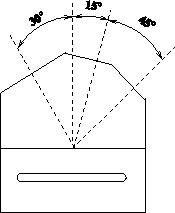
\includegraphics{figures/abb1.pdf}
    \caption{Schematische Darstellung des verwendeten Prismas mit den Winkeln $30 \,°$, $15 \,°$ und $45 \,°$ \cite{ap05}.}
    \label{fig:abb1}
\end{figure}